\iffalse
\let\negthickspace\undefined
\documentclass[journal,12pt,twocolumn]{IEEEtran}
\usepackage{cite}
\usepackage{amsmath,amssymb,amsfonts,amsthm}
\usepackage{algorithmic}
\usepackage{graphicx}
\usepackage{textcomp}
\usepackage{xcolor}
\usepackage{txfonts}
\usepackage{listings}
\usepackage{enumitem}
\usepackage{mathtools}
\usepackage{gensymb}
\usepackage{comment}
\usepackage[breaklinks=true]{hyperref}
\usepackage{tkz-euclide} 
\usepackage{listings}
\usepackage{gvv}                                        
\def\inputGnumericTable{}                                 
\usepackage[latin1]{inputenc}                                
\usepackage{color}                                            
\usepackage{array}                                            
\usepackage{longtable}                                       
\usepackage{calc}                                             
\usepackage{multirow}                                         
\usepackage{hhline}                                           
\usepackage{ifthen}                                           
\usepackage{lscape}
\setlength{\arrayrulewidth}{0.5mm}
\setlength{\tabcolsep}{18pt}
\renewcommand{\arraystretch}{1.5}
\newtheorem{theorem}{Theorem}[section]
\newtheorem{problem}{Problem}
\newtheorem{proposition}{Proposition}[section]
\newtheorem{lemma}{Lemma}[section]
\newtheorem{corollary}[theorem]{Corollary}
\newtheorem{example}{Example}[section]
\newtheorem{definition}[problem]{Definition}
\newcommand{\BEQA}{\begin{eqnarray}}
\newcommand{\EEQA}{\end{eqnarray}}
\newcommand{\define}{\stackrel{\triangle}{=}}
\theoremstyle{remark}
\newtheorem{rem}{Remark}
\begin{document}
\title{Progressions (7) 11.9.5}
\author{EE23BTECH11051-Rajnil Malviya}
\date{January 2024}
\maketitle
\subsection*{\textit{Question :-}}
If a function Satisfying f\brak {x+y} = f\brak{x} f\brak{y} for all $x,y \in {N}$ such that f\brak {1} =3 and $\sum_{x=1}^{n} f\brak{x} = 120$ , find the value of n .\\
\textit{Solution:- }
\fi
  $x=1$ and $y=1$ , we get
\begin{align}
    f\brak2&=f\brak{1+1}\\
     &={f\brak1} f\brak 1\\
     &=[f\brak 1]^2\\
      f\brak3&=f\brak{2+1} \\
  &    ={f\brak2} f\brak 1\\
 &= [f\brak 1]^3
        \end{align}
        Using induction , we get ;
       \begin{align}
            f\brak{x }&=[f\brak 1]^x\\
         r&=f\brak1\\
&=3
       \end{align}
    
\begin{table}[h!]
        \begin{tabular}{ | m{1.0cm} | m{1cm} |m{3cm} |} 
  \hline
 Symbol & Value &Description\\ 
 \hline
$x(0)$& 3 &first term \\
\hline
$r$& 3&common ratio   \\
\hline
$y\brak n$&120& sum of all n terms \\
\hline
$x(n)$& $ x \brak 0r^{n} u\brak n$&${n+1}^{th}$ term\\
\hline
\end{tabular}\\
\label{rajmal11.9.5.7}
\caption{}
    
    \end{table}

Refering from table ;
\begin{align}
X(z) &=\frac{3}{1-3z^{-1}} \quad \abs{z} > \abs{3}\\
Y(z) &= \frac{x(0)}{\brak{1-rz^{-1}}\brak{1-z^{-1}}} \quad \abs{z}> \abs{r}
\end{align}
Using partial differentiation 
\begin{align}
Y(z)&=\frac{x\brak0}{r-1}\brak{\frac{r}{1-r z^{-1}}-\frac{1}{1- z^{-1}}}  \quad \abs{z} > \abs{r}
\end{align}
applying inverse z transform ;
\begin{align}
y(n) &= x(0)\brak{\frac{r^{n+1}-1}{r-1}}u(n)\\
\implies 120 &= 3\brak{ \frac{3^{n+1}- 1}{3-1}}  \\
n &= 3
\end{align}
Ans . $n$ take values from $n=0$ to  $n=3$, so there are total four terms .
\newpage
\begin{figure}
   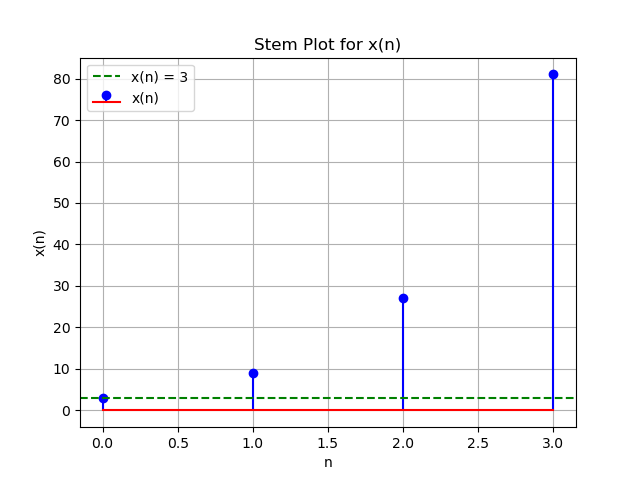
\includegraphics[width=1\linewidth]{ncert-maths/11/9/5/7/figs/i1.png}
\end{figure}
\begin{figure}
   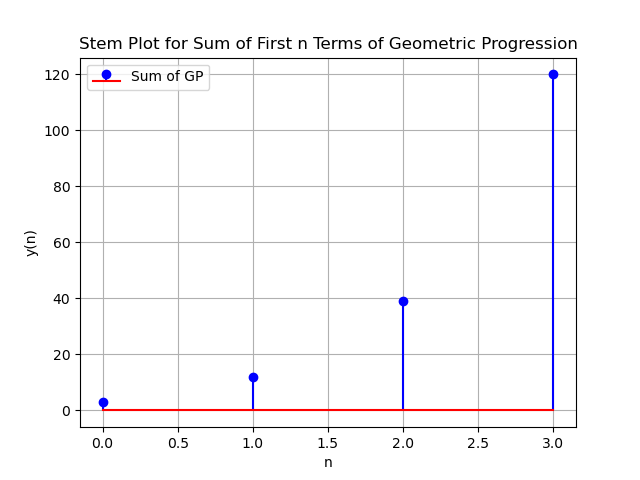
\includegraphics[width=1\linewidth]{ncert-maths/11/9/5/7/figs/i2.png}
\end{figure}
%\end{document}
